\subsection{2026-09-21 --- EDA round 3b: point-in-time correctness and temporal transforms}
\label{sec:eda-round-3b}

Round 3a (Section~\ref{sec:eda-round-3}) under-covered the time-series side --- it tested three
hypotheses and refuted two, rather than surveying transformations --- and it contained a
point-in-time error. This entry fixes both. Notebook:
\texttt{src/EDA/eda\_round3b\_temporal.ipynb}.

\subsubsection*{What the documentation actually specifies about test-time availability.}
The task PDF lists input \emph{categories} and states that predictions go to Kaggle. It says
\textbf{nothing} about temporal availability rules. Earlier claims in this log about what is
``available at test time'' were therefore inference, not documented fact. The question is
answerable empirically, so it was checked.

\finding{\textbf{(0, verified)} Every \emph{feature} file extends past the last hour we must
predict (2024-12-31 23:00): price to 2025-12-31, inflow to 2025-10-15, volume and water value to
2025-01-01, both constraint files to 2025-12-31. So all feature sources are genuinely available
for all 725 test cases. \textbf{Labels stop at 2022-12-31}, so any feature derived from past
\emph{targets} --- trailing ON-rate, previous case's decisions --- is unusable beyond the first
test case. The terminal (day$+$8) water value is available for \textbf{724 of 725} cases; only the
final case (2024-12-25) reaches past the file's end and needs a documented fallback.}

\medskip\noindent
A distinction the earlier draft got wrong: \emph{beyond-horizon} future prices (e.g.\ hour 200
when the case ends at 167) are \textbf{permitted} --- nothing forbids them and on a fixed test set
they are not cheating. The only argument against them is that the label-generating optimizer
never saw past its own horizon, so such features describe information the target does not depend
on. That is a modelling judgement to test, not a correctness rule; round 3a overstated it as the
latter.

\subsubsection*{Corrected lead/lag.}

\begin{figure}[htbp]
  \centering
  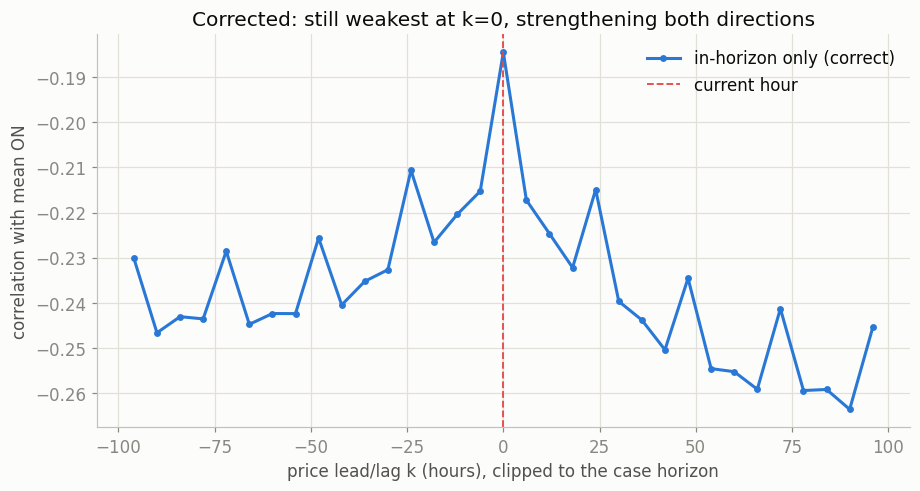
\includegraphics[width=0.75\linewidth]{figures/eda3b_01_leadlag_corrected.png}
  \caption{Price lead/lag correlation, clipped to the case horizon.}
  \label{fig:eda3b-leadlag}
\end{figure}

\finding{\textbf{(1, corrects round 3a finding 3)} Round 3a's lead/lag curve ignored case
boundaries --- for a row at hour 160, $k=+90$ reached 82 hours past the horizon end. Recomputed
within the horizon: $-0.230$ at $k=-96$h, $-0.185$ at $k=0$, $-0.245$ at $k=+96$h. The
qualitative conclusion \textbf{survives} (signal weakest at the current hour, strengthening both
directions) but round 3a's reported peak of $-0.273$ was inflated; the correct magnitude is
$\approx -0.245$.}

\subsubsection*{Temporal transforms on the fast series (price).}

\begin{figure}[htbp]
  \centering
  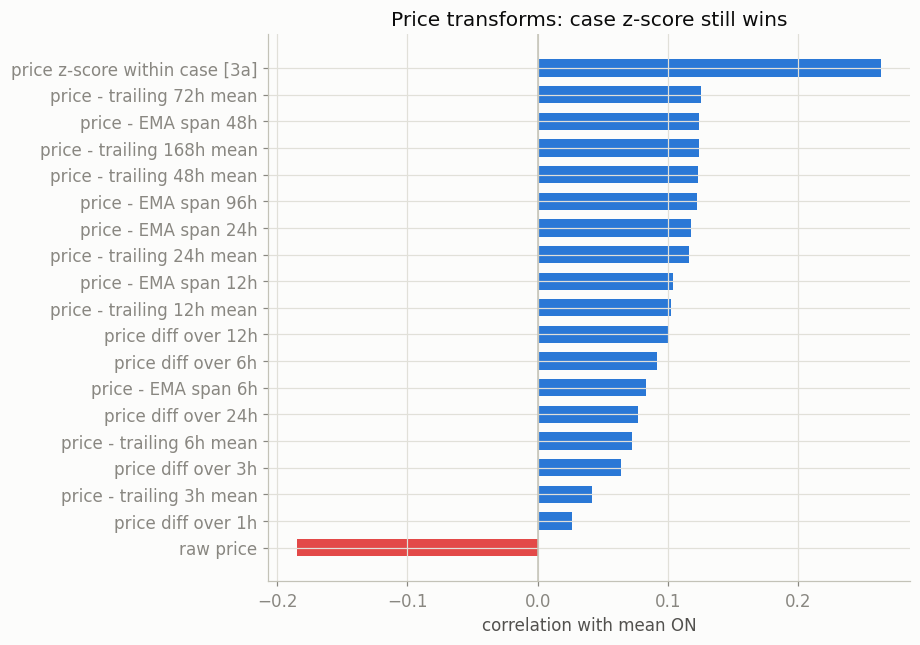
\includegraphics[width=0.75\linewidth]{figures/eda3b_02_price_transforms.png}
  \caption{Seventeen price transformations ranked by correlation with mean ON.}
  \label{fig:eda3b-price}
\end{figure}

\finding{\textbf{(2)} Trailing-window and EMA relative-price features do flip the sign of the
raw-price relationship --- best are \texttt{price $-$ trailing 72h mean} ($+0.125$) and
\texttt{price $-$ EMA span 48h} ($+0.124$) --- but all are \textbf{roughly half as strong as the
within-case z-score} ($+0.263$). Diffs and momentum are weakest ($+0.03$ to $+0.10$, peaking at a
12h lag). \textbf{For fast series, normalise against the case, not a rolling window} --- the case
is the window the optimizer actually solved over.}

\subsubsection*{Temporal transforms on the slow series --- the strongest \emph{correlation} so far.}

\begin{figure}[htbp]
  \centering
  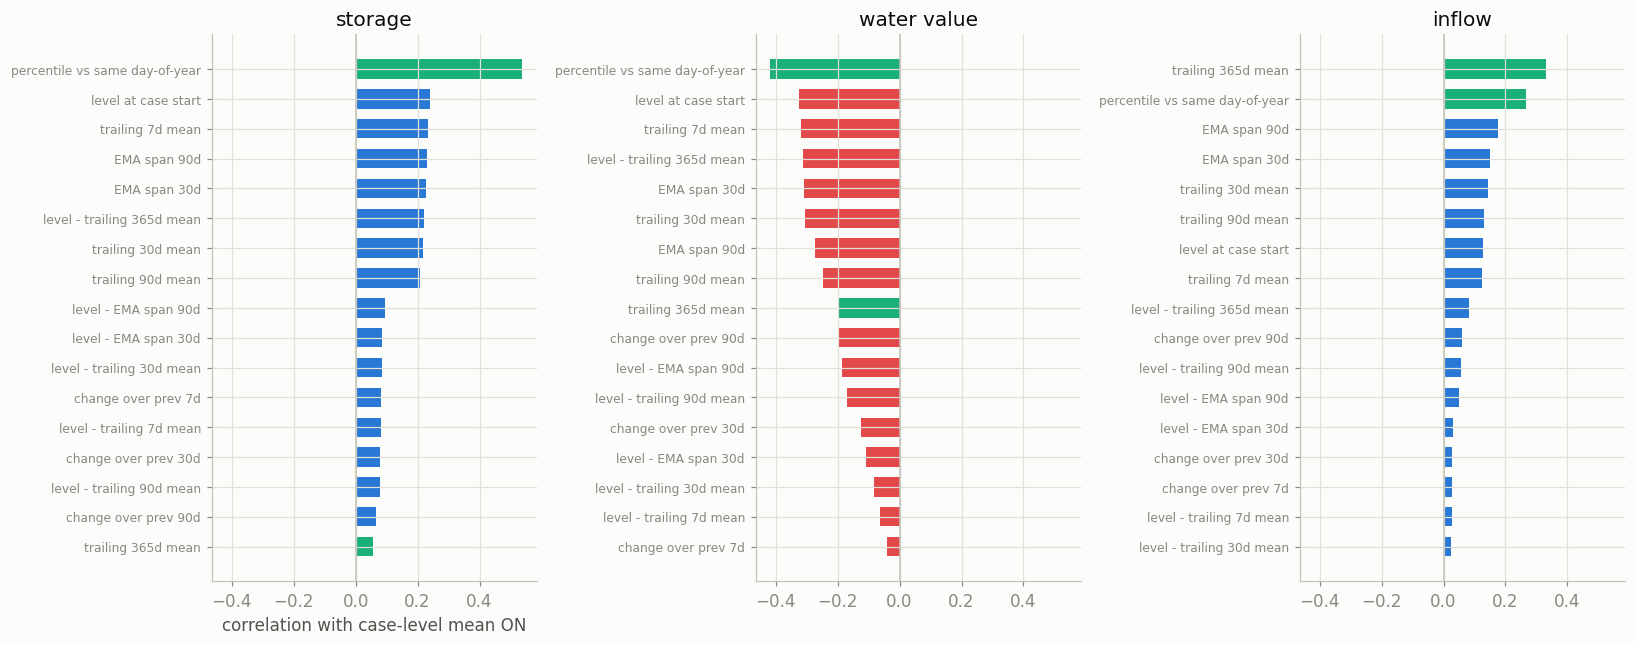
\includegraphics[width=0.98\linewidth]{figures/eda3b_03_slow_series_transforms.png}
  \caption{Seventeen transforms each on storage, water value and inflow (all backward-looking).}
  \label{fig:eda3b-slow}
\end{figure}

\finding{\textbf{(3)} Normalising the slow series against \emph{the same time of year} transforms
them (Figure~\ref{fig:eda3b-slow}):
\begin{center}
\begin{tabular}{lrrr}
\toprule
Series & Raw level & Best transform & Gain \\
\midrule
Storage     & $+0.241$ & percentile vs.\ same day-of-year: $\mathbf{+0.537}$ & 2.2$\times$ \\
Water value & $-0.325$ & percentile vs.\ same day-of-year: $\mathbf{-0.417}$ & 1.3$\times$ \\
Inflow      & $+0.128$ & trailing 365d mean: $\mathbf{+0.331}$ & 2.6$\times$ \\
\bottomrule
\end{tabular}
\end{center}
Storage's seasonal percentile ($\mathbf{+0.537}$) is \textbf{the strongest correlation measured
anywhere in this project}, well ahead of the price z-score ($+0.263$) that was previously our
best candidate. The mechanism is simple: absolute storage confounds season --- every reservoir is
full in June and drawn down in April --- so ``is this reservoir unusually full \emph{for the time
of year}'' isolates the scarcity signal that drives scheduling. Inflow's trailing 365-day mean is
the same idea over a longer window: the wet-year/dry-year regime.}
\supersededby{sec:feature-iter-1}{this correlation did not survive model testing --- the seasonal percentile made the score \emph{worse} ($-0.020$, 0/4 folds).}

\finding{\textbf{(4)} Diffs, momentum and EMAs are consistently weak on the slow series too
($-0.20$ to $+0.08$), and EMAs land within noise of plain trailing means. Neither earns priority
over the seasonal normalisations. All transforms in this section are strictly backward-looking
and therefore point-in-time safe.}

\subsubsection*{The rule that emerges.}
\textbf{For fast series, normalise against the case. For slow series, normalise against the
season.} Diffs, momentum and EMAs underperform both. \texttt{report/feature\_backlog.md} has been
reordered accordingly --- the seasonal-percentile family is now the top-priority iteration, ahead
of the price normalisations.
